\chapter{Implementation}\label{chap:implementation}
\section{FPGAs}
This thesis started with the fpga-zynq repository \cite{github_fpga_zynq}
which provides a version locked edition of the rocket-chip repository,
a Linux front-end which enables us to communicate with the RISC-V core on the FPGA
and rocket-chip build configurations for the interconnect between the front-end and
the RISC-V processor. The project is deprecated, and thus the functionality
might be limited.

\subsection{Xilinx Zybo Zynq-7000}
The first attempt was to put the rocket chip Verilog code on the FPGA of
a Xilinx Zybo Zynq-7000 with the Xilinx Vivado software.
The Xilinx Zybo board combines an FPGA with 28,000 logic cells with
an ARM dual-core \cite{xilinx_zybo}.
The rocket-chip fpga-zynq configuration from the project defines
the following code:
\begin{lstlisting}[language=scala, frame=single]
    ...
    class ZynqSmallConfig extends Config(
        new WithZynqAdapter ++
        new DefaultSmallConfig
    )
    ...
\end{lstlisting}
The configuration creates a small rocket-core with an attached
ZynqAdapter, which uses the Xilinx AXI4 protocol to communicate with
the ARM cores.

After compiling the rocket-chip Verilog code with the
Xilinx Vivado suite to a binary, the software reported that the
design would not fit on the Zybo board.
The number of logic cells of the board was not high enough, although
the repository states compatibility with the Zybo board in the
repository description.

\subsection{Xilinx Zedboard}
The Zedboard by Xilinx was the next larger board which was available at the
chair of operating systems at the Technical University Munich.
It houses 85,000 logic cells \cite{elinux_zedboard} 
and could be programmed with the rocket chip design.
After the compilation of the design, one needs to prepare an SD card, which
contains all files the Zedboard needs to boot.
Normally all of these files can be obtained by executing the
download scripts in the fpga-zynq repository but as the project is
deprecated some files are missing or are no longer valid.
The Linux kernel and the U-boot (the boot manager
for the project) had to be manually compiled as they were no longer available.
Also, the integrated RISC-V compiler in the Xilinx suite
is deprecated and needs to be replaced with \textit{riscv64-unknown-elf-gcc}
from the compiled version of the risc-toolchain \cite{github_risc-v_toolchain}.
In general, it was not easy to follow the tutorials as many things
were deprecated, steps were missing, files were no longer available, and
links lead to 404 pages.
After everything was put in place on the SD card, the Zedboard would not
boot past the U-boot bootloader.
Even combined efforts with other colleges from the chair and
multiple RAM load configurations could not get the boot process past
the u-boot command line.
In the issues tab of the fpga-zynq repository multiple users report
that they have difficulties to get the project running
\footnote{\url{https://github.com/ucb-bar/fpga-zynq/issues/92}}\textsuperscript{,}
\footnote{\url{https://github.com/ucb-bar/fpga-zynq/issues/97}}\textsuperscript{,}
\footnote{\url{https://github.com/ucb-bar/fpga-zynq/issues/101}\label{foot:fpga-zynq_issue101}}.
The user zxhero speculates that the problem might be the communication
between the rocket-chip and the debug module
\footref{foot:fpga-zynq_issue101}.
It is certainly possible to bring a Rocket core on the Zedboard,
but this requires greater efforts, which are out of the scope of
this thesis. The connection problems might
also be connected to the issue "AXI4 MEM port: wrong write address timing"
in the rocket-chip repository
\footnote{\url{https://github.com/freechipsproject/rocket-chip/issues/1778}}.

\subsection{Xilinx Arty A7: Artix-7}
After some research, the next best option to get a running rocket-chip
core on an FPGA was the Xilinx Arty A7: Artix-7.
The board features only an FPGA which eliminates the previously problematic
AXI4 ZynqAdapter between the FPGA and the ARM processor and replaces it
with a simple JTAG connector.
It is used by SiFive to prototype their first RISC-V microcontroller, the HiFive1.
SiFive created the Freedom platform on GitHub with configuration files
and additional extensions to make the setup of the board
easier \cite{github_freedom}.
Although the setup of the Freedom platform was easier and much more
up-to-date than the fpga-zynq project, some parts were still missing.
An alternative complete guide 
\footnote{\url{https://github.com/Mixermachine/setup-freedom-e300-on-arty-A7}}
on how to set up the Freedom E300 platform from SiFive on the
Xilinx Arty A7 board was created, to help future projects.
All problems that occurred during
the setup and how to mitigate them are listed in the guide.
After the setup, the board booted the rocket core without problems,
and the integrated programs can be run.
However, upon further inspection of the rocket core, it came apparent,
that the version for the Arty board will not be sufficient for this
Bachelor thesis. One can spot this in the Chisel configuration:
\begin{lstlisting}[language=scala, frame=single]
    class DefaultFreedomEConfig extends Config (
        ...
        new WithJtagDTM ++
        new TinyConfig
    )
\end{lstlisting}
The configuration defines the core to be "tiny", which sets the "useVM" boolean
to false and thus disables the creation of the MMU, which is essential
for the Checkpoint/Restore approach described in chapter \ref{chap:concept}.
As the E300 platform is not usable for this thesis and larger FPGAs are
very costly (the larger SiFive U500 platform use the Xilinx Virtex-7 FPGA
VC707, which costs about 3,500 dollar \cite{github_freedom},
\cite{xilinx_virtex7}), further steps are done in the simulator.

\section{Rocket-chip} \label{sec:rocket-chip}
The rocket-chip repository on GitHub is often denoted as "cutting-edge"
and currently has some build issues
\footnote{\url{https://github.com/freechipsproject/rocket-chip/issues/1709}}\textsuperscript{,}
\footnote{\url{https://github.com/freechipsproject/rocket-chip/issues/1644}}.
The release feature of GitHub is also not used by the rocket-chip repository, 
so finding a stable version might not always be easy.
In the following sections the referenced rocket-chip version of the freedom
repository \textit{b21c7879b3ea22f69cb8457109561f37c225f8ea} is used, as it
seems to be stable.
To clone the repository we need to execute the following code:
\begin{lstlisting}[language=bash, frame=single]
    # Checkout the repository and the connected submodule
    git clone https://github.com/sifive/freedom.git
    cd freedom
    git submodule update --init --recursive
    
    # Build the included version of the RISC-V GNU Compiler Toolchain
    cd rocket-chip
    mkdir toolchain
    cd toolchain
    export RISCV=\$(pwd)
    cd ../riscv-tools/
    ./build.sh
    cd ..
    
    # To run Verilater simulation tests we need to build Verilator and the tests
    cd emulator
    # if we need waveform output add the prefix 'debug' to make
    make    
\end{lstlisting}
The bash commands above will download the source code, compile the compiler toolchain
and the test suite with the Verilog simulator Verilator.
Verilator compiles Verilog code to C or C++ code \cite{verilator_verilator}.
After we compiled the test suite, we will find \textit{.riscv} files that contain
the tests.

\subsection{Finding the MMU}
As the approach of this thesis on Checkpoint/Restore heavily relies on the memory
management unit it is critical to find the code for the MMU.
The rocket-chip code does not contain any class that is labeled "MMU" and does contain
in general nearly no comments, which made it hard to find references to the actual
position of the MMU.
After consulting the mailing list, first a hint to the Translation Lookaside Buffer (TLB)
Scala file was given by Bruce Holt
\footnote{\url{https://groups.google.com/a/groups.riscv.org/forum/?utm_medium=email&utm_source=footer\#!msg/isa-dev/vf33dd6ulh0/mu3AaPTvDQAJ}}.
A second hint was given by Abraham Gonzalez and Farzad Farshchi
\footnote{\url{https://groups.google.com/forum/?utm_medium=email&utm_source=footer\#!msg/riscv-boom/jZ1gC4Qs35Q/8HltWll_CgAJ}}.
They recommended to
\begin{itemize}
    \item read the documentation at
    \footnote{\url{https://github.com/cnrv/rocket-chip-read}}\textsuperscript{,}
    \footnote{\url{https://www.lowrisc.org/docs/tagged-memory-v0.1/rocket-core/}}.
     \item build the Verilog and open it in a schematic viewer
     \item run 'risc-v tests' and look into the waveform
     \item read section 4.3 and 4.4 of the privileged spec
\end{itemize}
and mentioned, that the MMU in the rocket-chip project is called page table
walker (PTW). A quick search in the project revealed the file
\textit{rocket-chip/src/main/scala/rocket/PTW.scala} to be the object of desire.
It contains classes like 
\textit{PTWReq (PTW request), PTWResp (PTW response), TLBPTWIO (TLB PTW communication)}
and one particularly interesting class \textit{PTE (page table entry)}
\begin{lstlisting}[language=scala, frame=single]
    class PTE(implicit p: Parameters) extends CoreBundle()(p) {
        val ppn = UInt(width = 54)
        val reserved_for_software = Bits(width = 2)
        val d = Bool()
        val a = Bool()
        val g = Bool()
        val u = Bool()
        val x = Bool()
        val w = Bool()
        val r = Bool()
        val v = Bool()
        
        def table(dummy: Int = 0) = v && !r && !w && !x
        def leaf(dummy: Int = 0) = v && (r || (x && !w)) && a
        def ur(dummy: Int = 0) = sr() && u
        def uw(dummy: Int = 0) = sw() && u
        def ux(dummy: Int = 0) = sx() && u
        def sr(dummy: Int = 0) = leaf() && r
        def sw(dummy: Int = 0) = leaf() && w && d
        def sx(dummy: Int = 0) = leaf() && x
    }
\end{lstlisting}
The class PTE defines one page table entry, but no comment is given in
the definition. In general, comments in the project are quite sparse,
the 385 lines \textit{PTW.scala} file contains only five comments.
After some research, the variables could be resolved with the
help of the RISC-V Privileged ISA Specification
\cite[p.~59-61]{risc-v_isa_manual_priviliged_arch}.
"Virtual page" is abbreviated by vp.
\begin{itemize}
    \item d: Dirty, vp has been written
    \item a: Accessed, vp has been read, written or fetched
    \item g: Global, vp exists in all address spaces
    \item u: User, vp is accessible to the user mode
    \item x: Executable, vp is executable
    \item w: Writable, vp is writeable
    \item r: Readable, vp is readable
    \item v: Valid, vp is valid
    \item table: vp is pointer to next level of page table.
    \item leaf: vp is valid, at least fetched and can be read or executed
    \item ur: vp is sr and readable by user
    \item uw: vp is sw and writable by user
    \item ux: vp is sx and executable by user
    \item sr: vp is leaf and readable
    \item sw: vp is leaf, writable and dirty
    \item sx: vp is leaf and executable
\end{itemize}
To help future developers, a fork and a new branch of the project has been
created on GitHub which adds comments to the definitions of the \textit{PTW.scala} file
\footnote{\url{https://github.com/Mixermachine/rocket-chip/blob/documentation/commentsPTW/src/main/scala/rocket/PTW.scala}}.
The patches will be packed into a patch and submitted to the original
project in a pull request.
Now that we know where the PTW is defined we need to find out how it works.
A first hint on how the PTW is connected with the TLB can be seen in figure
\ref{fig:lowrisc_icache} from the lowRISC project.
\begin{figure}
    \centering
    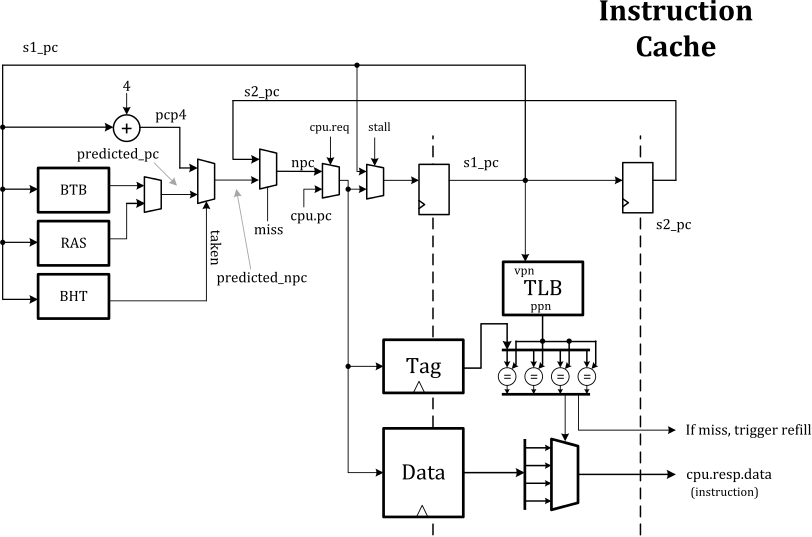
\includegraphics[width=0.9\textwidth]{figures/lowrisc_icache}
    \caption{Schematic of the instruction cache of a Rocket core
        \cite{lowrisc_rocket_core_overview}}
    \label{fig:lowrisc_icache}
\end{figure}
The figure shows the L1 instruction cache of a Rocket core.
On the right side of the schematic, we can see that a TLB element
is built directly into the Cache module, most certainly to speed up
the lookup of frequently used virtual pages. This TLB can trigger
a refill which is fulfilled by the PTW. For the further setup of the system a question regarding the setup of the TLB and PTW on the mailing list
was asked 
\footnote{\url{https://groups.google.com/a/groups.riscv.org/forum/?utm_medium=email&utm_source=footer\#!msg/hw-dev/_RqboAwU8pQ/T8rvsE6eGAAJ}}.
Andrew Waterman replied to the inquiry and clarified the setup:
The Rocket core is connected over the L1 instruction cache to the
TLB that resolves often requested PTEs. If the TLB does not have
a specific entry, it forwards the request to the PTW.
The Rocket core also has a direct connection to the PTW, but this
is only used to get the page-table base register.
This register is responsible for providing each process with a
separated logic address space
\cite["Page Tables" -> "The PTBR"]{uniminnesota_vm_address_translation}.
The L1 data cache has a similar TLB element.
The PTW has a small cache for nonleaf nodes (pointer to other
page tables) and a larger L2 TLB for PTEs.

\subsection{Thoughts on the implementation of the concept}
\label{subsec:thoughs_impl}
The RISC-V setup of cascaded TLBs certainly provides faster address resolution
but makes the implementation of the Checkpoint/Restore concept from chapter
\ref{chap:concept} harder.

\subsubsection{L1 cache}
The complete Checkpoint/Restore algorithm implementation could
happen directly in the L1 caches, as this is the first location a checkpointed
PTE would hit a possible resolution. This approach is beneficial in regards
to the execution performance, as every processor would be connected to
its own Checkpoint/Restore element. The downside is that this approach would
enlarge the die size of the Cache memory. L1 cache is extraordinarily
expensive to build, as it needs to run at high clock speeds.

\subsubsection{PTW}
A more cost-effective approach would be to implement the mechanism mainly
in the PTW. A checkpointed PTE then would first need to be processed
in the PTW, which then needs to either synchronize or invalidate
all existing copies in the TLBs.
In regard to the TLBs there are multiple possible solutions.
The TLBs in the standard form do not know how to handle checkpointed
PTEs.
\begin{itemize}
    \item TLBs do not store checkpointed PTEs
    \item TLBs get a changed PTE with different physical address
    \item TLBs contain a minimal Checkpoint/Restore logic
\end{itemize}

The first solution is the cheapest one but could hurt the performance
of the system, as all checkpointed PTEs can no longer be cached in
the L1 cache and every operation needs to be performed by the PTW.

In the second solution the PTW invalidates all previous copies
of PTEs in the L1 Caches and then replaces them with manipulated
PTEs. This PTEs would still have the virtual address out of the 
first virtual memory block (prefix 0) but the physical address
points to the new working copy.

The last solution would need a change in the TLBs. A minimal
Checkpoint/Restore logic could be implemented, which only handles
the CA, CW bits in the PTEs. The rest of the logic for creating
and managing checkpoints can be outsourced to the PTW.
A new \textit{PTWResp} format might be necessary as the TLBs need to receive
multiple PTEs for one \textit{PTWReq} in order to process a checkpoint
correctly.\newline

Due to time constraints, this thesis can not go further in the implementation
of the concept.

\subsection{riscv-tests}
For future efforts in the direction of implementing the Checkpoint/Restore
concept of this thesis
or in general to understand the logic of the processor better the riscv-tests
repository is beneficial, as the simulation can output waveform files which
contain all wire states of the CPU run.
The riscv-tests system \cite{github_riscv-tests} is designed to be as modular as possible.
The included test virtual machine (TVM) hides the differences between
the implementations by restricting the operation of the test.
The TVM can define:
\begin{itemize}
    \item The set of registers and instructions that can be used.
    \item Which portions of memory can be accessed.
    \item The way the test program starts and ends execution.
    \item The way that test data is input.
    \item The way that test results are output.
\end{itemize}
\cite{github_riscv-tests} \newline
Currently, the following TVMs are already implemented.
All of them feature only one hardware thread:
\begin{itemize}
    \item rv32ui: RV32 user-level, integer only
    \item rv32si: RV32 supervisor-level, integer only
    \item rv64ui: RV64 user-level, integer only
    \item rv64uf: RV64 user-level, integer and floating-point
    \item rv64uv: RV64 user-level, integer, floating-point, and vector
    \item rv64si: RV64 supervisor-level, integer only
    \item rv64sv: RV64 supervisor-level, integer and vector
\end{itemize}
\cite{github_riscv-tests} \newline
An additional layer of testing flexibility is added with the
target environment configuration:
\begin{itemize}
    \item p: virtual memory is disabled, only core 0 boots up
    \item pm: virtual memory is disabled, all cores boot up
    \item pt: virtual memory is disabled, timer interrupt fires every 100 cycles
    \item v: virtual memory is enabled
\end{itemize}
\cite{github_riscv-tests} \newline
Testing programs are written in an assembly language, which includes the RISC-V ISA
and additional commands for the test environment like
\textit{RVTEST\_CODE\_BEGIN, RVTEST\_PASS, RVTEST\_CODE\_END, and RVTEST\_FAIL}.
A nice example is the following assembly code take from \cite{github_riscv-tests}.
\begin{lstlisting}[frame=single]
    #include "riscv_test.h"

    RVTEST_RV64U        # Define TVM used by the program.
    
    # Test code region.
    RVTEST_CODE_BEGIN   # Start of test code.
            lw      x2, testdata
            addi    x2, 1         # Should be 42 into \$2.
            sw      x2, result    # Store result into memory overwriting 1s.
            li      x3, 42        # Desired result.
            bne     x2, x3, fail  # Fail out if doesn't match.
            RVTEST_PASS           # Signal success.
    fail:
            RVTEST_FAIL
    RVTEST_CODE_END     # End of test code.
    
    # Input data section.
    # This section is optional, and this data is NOT saved in the output.
    .data
            .align 3
    testdata:
            .dword 41
    
    # Output data section.
    RVTEST_DATA_BEGIN   # Start of test output data region.
            .align 3
    result:
            .dword -1
    RVTEST_DATA_END     # End of test output data region.
\end{lstlisting}
At the start of the program, the \textit{riscv\_test.h} header file needs
to be included, which defines the macros that are used by the TVM.
After the include, we define the TVM which should be used for our test.
In the test run, we load some test data (32-bit unsigned integer 41) and
add 1 to it. The reasonable answer for this calculation is of course 42, which is
checked in the test by comparing the two registers x2 and x3.
If this check does for some reason fail, we jump to RVTEST\_FAIL which triggers
the failure of the test.
This test can be used to get to know the PTW better, as the command \textit{sw}
stores the register value in the memory.
Maybe a reduced version that only executes:
\begin{lstlisting}[frame=single]
    #include "riscv_test.h"
    
    RVTEST_RV64U
    
    RVTEST_CODE_BEGIN
        lw      x2, testdata
        sw      x2, result
        RVTEST_PASS
    RVTEST_CODE_END
    testdata:
        .dword 42
\end{lstlisting}
might be a good place to start.
